\documentclass[11pt]{article}
\pdfminorversion=7
\usepackage[margin=1in]{geometry}
\usepackage{graphicx}
\usepackage{amsmath, amssymb}
\usepackage{float}
\usepackage{hyperref}
\usepackage{caption}
\usepackage{subcaption}
\usepackage{fancyhdr}
\usepackage{booktabs}
\usepackage{tikz}
\usepackage{authblk}
\usepackage{titlesec}
\usepackage[style=apa, backend=biber]{biblatex}
\usepackage{tikz}
\usepackage{etoolbox}
\addbibresource{references.bib}


\usepackage{tikz}
\usetikzlibrary{arrows.meta, positioning}



\titleformat{\section}{\large\bfseries}{\thesection.}{1em}{}
\titleformat{\subsection}{\normalsize\bfseries}{\thesubsection.}{1em}{}

\setlength\parskip{6pt}
\setlength\parindent{0pt}

\pagestyle{fancy}
\fancyhf{}
\rhead{\thepage}
\lhead{ViTs vs. CNNs in Brain Tumor MRI Detection}

\title{\textbf{A Comparative Evaluation of CNN and Vision Transformer Architectures for Brain Tumor Detection in MRI Scans}}
\author{Zain Aboobacker}
\affil{Natick High School}
\date{\today}

\begin{document}
\maketitle

\begin{abstract}
This study evaluates the performance of convolutional neural networks (CNNs) and Vision Transformers (ViTs) in classifying various brain MRI scans for the detection of tumors. Model series such as EfficientNet, ConvNeXt, ViT, and SwinTransformer were trained on a publicly available multiclass brain tumor dataset. To support experimentation and reproducibility, a custom GUI-based deep learning software was developed, enabling users to train models, configure parameters, apply data augmentation, monitor performance metrics, and generate diagnostic reports. A comparative analysis was conducted using accuracy, precision, recall, F1-score, AUROC, and confusion matrices. Results showed that ViT-B/16, EfficientNetB0, and ViT-B/32 achieved test accuracies of over 98~\%. ViT-B/16 performed the best overall, demonstrating that larger model capacity and reduced patch size enhance feature extraction in brain MRI classification. EfficientNetB0 delivered strong performance despite its reduced complexity, demonstrating the strength of CNNs and the potential of transformer-based architectures for detecting brain tumors.
\end{abstract}

\section{Introduction}

Brain tumor detection with MRI scans is highly crucial for early treatment and diagnosis in medicine. However, manual evaluations of MRI scans are time-consuming and may be prone to error. This research explores the possibilities of using convolutional neural networks (CNNs), vision transformers (ViTs), and hybrid CNN-Transformer models in the automation of brain tumor detection images with an additional goal of creating a user-friendly deep learning platform for model training and diagnostics. 

Despite the promising potential of the automation of tumor detection, many are skeptical due to risks associated with false negatives and positives, and the severe consequences that may come from it. This research aims to analyze the plausibility of these risks by evaluating multiple deep learning models on brain MRI data using accuracy, precision, recall, F1-score, AUROC, and confusion matrices. This study assesses the reliability and diagnostic consistency of AI-based systems in medical applications with a particular focus on brain tumor classification.

In recent years, CNNs have demonstrated strong performance in detecting abnormalities in a plethora of image scans such as X-rays, CT scans, and MRIs. However, most systems require significant technical expertise to operate. These limitations prevent accessibility to researchers and clinicians without the required background. Vision Transformers (ViTs) are a relatively newer class of models originally designed for natural classification; however, they have shown competitive results in medical images, but remain underexplored in clinical windows. This research contributes to the medical field by directly comparing several CNN and ViT architectures and integrating them into an intuitive interactive platform. By providing performance benchmarks and a practical interface, this study aims to advance the deployment of AI tools in radiological diagnostics.

Additionally, a user-friendly deep learning application was developed, allowing users to load datasets, configure training parameters, monitor real-time performance, and export evaluation results and diagnostic reports. The application allows users to select multiple model architectures and requires no coding knowledge. The interface enables streamlined experimentation and diagnostics for users without extensive background knowledge.

\section{Related Works}

Deep learning has received significant traction in medical imaging due to its ability to recognize complex patterns in data, allowing accurate diagnosis and detection of subtle anomalies in medical scans. Convolutional neural networks (CNNs), in particular, have been widely applied to MRI classification tasks  in recent studies. 

\textcite{albalawi2024enhancing} developed a custom 25-layer CNN for multiclass brain tumor classification on a dataset of over 7,000 MRI images and achieved an accuracy of 99~\%. This significantly outperformed earlier methods, demonstrating the strong feature extraction and classification of CNNs for medical images.

Within the same domain, \textcite{zarenia2025automated} suggested a hybrid CNN model with a hierarchical multiscale deformable attention module (MS-DAM) to classify brain tumors across 14 classes. Their model, which achieved an accuracy of more than 96.5\%, had a segmentation module built in, an end-to-end solution for detection and localization in brain MRI.

Additionally, \textcite{mahmud2023cnn} made a comparison between lightweight CNNs and typical deep architectures like ResNet and VGG, with the conclusion being that simpler CNNs can also produce high accuracy if well optimized for brain MRI classification.

Although CNNs have exhibited strong performance, vision transformers (ViTs) remain relatively unexplored in medical imaging. Recent studies, however, highlight their potential. \textcite{reddy2024ftvt} explored the application of fine-tuned ViT (FTVT) models for four-class brain tumor classification using a similar dataset to that of \textcite{albalawi2024enhancing}. Their best model, FTVT-l16, achieved a classification accuracy of 98.70\%, also demonstrating the effectiveness of transformer-based models in medical diagnosis.

Similarly, \textcite{poornam2024vitalt} introduced VITALT, a rotation-invariant Vision Transformer architecture for brain tumor classification. VITALT was trained across four MRI datasets and achieved accuracy above 98.8~\%, demonstrating the strength of ViTs when rotational variance is taken into account.

Hybrid CNN-VITs have also demonstrated promising performance in the field of medical imaging. \textcite{karagoz2024resvit} introduced ResViT, a hybrid CNN–ViT model pre-trained using self-supervised contrastive learning. On the BraTS and Kaggle MRI datasets, ResViT achieved over 98.4~\% accuracy.

These works demonstrate the effectiveness of CNNs, ViTs, and CNN-ViT hybrid models for brain MRI classification. However, most existing research requires advanced expertise and lacks integrated tools for non-expert users. This project addresses that gap by performing a comparative evaluation on a range of CNN and ViT models while also introducing a user-friendly interface for model training, evaluation, and diagnostic reporting.

\section{Dataset and Preprocessing}

The dataset used in this study consists of brain MRI scans for brain tumor classification. It includes four classes: glioma, meningioma, pituitary, and no tumor. The images were sourced from a publicly available Kaggle dataset, containing a total of 7,022 images evenly distributed across the classes. The dataset was split into training and testing sets using an 80/20 ratio.

\subsection*{Image Standardization}

To ensure consistency in input dimensions across all models, each MRI image was resized to a fixed resolution of $224 \times 224$ pixels. This resizing operation can be formalized as a mapping function:

\[
R: \mathbb{R}^{H \times W \times C} \rightarrow \mathbb{R}^{224 \times 224 \times C}
\]

where $H$, $W$, and $C$ represent the original height, width, and number of channels of the input image, respectively. This transformation enforces spatial uniformity across the dataset and aligns with input size requirements of pretrained CNNs and transformer-based models. 

Following resizing, all images were normalized to zero mean and unit variance using the following channel-wise transformation:

\[
x' = \frac{x - \mu}{\sigma}
\]

where $x$ denotes the original pixel intensity, $\mu$ is the mean, and $\sigma$ is the standard deviation for each channel. In this study, $\mu = \sigma = 0.5$ were used for all RGB channels, scaling pixel values from the $[0, 1]$ range to $[-1, 1]$:

\[
x' = \frac{x - 0.5}{0.5}
\]

This normalization improves numerical stability and accelerates model convergence during training.

\subsection*{Data Augmentation}

To enhance generalization and reduce overfitting, data augmentation was applied to the training images using stochastic transformations. These augmentations simulate natural variations in MRI acquisition, such as orientation, position, and scanner-induced artifacts, while preserving semantic content. The following techniques were used:

\begin{itemize}
\item \textbf{Random Horizontal Flip}: Applied with probability $p = 0.5$, flipping the image along the vertical axis:
\[
x' = \text{Flip}_H(x) \quad \text{if } u < 0.5, \quad u \sim \mathcal{U}(0, 1)
\]

\item \textbf{Random Affine Transformation}: Applied with probability $p = 0.5$, A composite transformation involving small random rotations, translations, and scaling:
\[
T(x) = A_{\theta, s, t}(x)
\]
where $\theta \in [-15^\circ, 15^\circ]$ is the rotation angle, $s \in [0.95, 1.05]$ is the scaling factor, and $t$ is a translation vector with magnitude up to 5\% of the image dimensions.

\item \textbf{Gaussian Blur}: A convolutional smoothing operation applied with probability $p = 0.2$:
\[
x' = x * G_{\sigma}
\]
where $G_{\sigma}$ is a 2D Gaussian kernel with standard deviation $\sigma \in [0.1, 0.5]$ and fixed kernel size of 3.
\end{itemize}

These augmentations were applied dynamically during training, introducing slight variations at each epoch to improve the model's robustness to real-world imaging noise and spatial distortions.

\begin{figure}[H]
\centering
\begin{subfigure}[b]{0.45\textwidth}
\centering
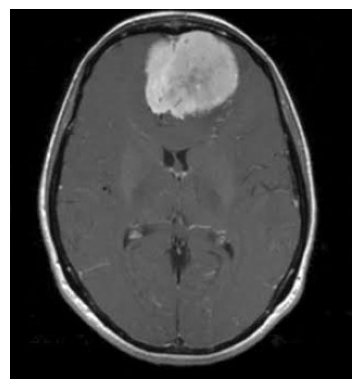
\includegraphics[width=\textwidth]{figures/normal_img.png}
\caption{Sample MRI without Data Augmentation and Normalization}
\label{fig:image1}
\end{subfigure}
\hfill
\begin{subfigure}[b]{0.45\textwidth}
\centering
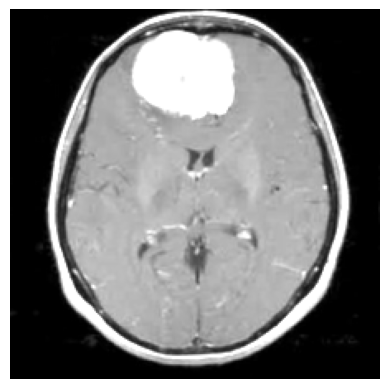
\includegraphics[width=\textwidth]{figures/transformed_img.png}
\caption{Sample MRI with Data Augmentation and Normalization}
\label{fig:image2}
\end{subfigure}
\caption{Example MRI images with and without Data Augmentation / Normalization}
\label{fig:sample_mris}
\end{figure}


\section{Methodology}
This section outlines the experimental framework used to accurately compare the performance of Convolutional Neural Networks and Vision Transformers in the task of brain tumor classification. The methodology includes a standardized classification head, model selection, training strategy, and evaluation metrics. All models were trained using the same dataset, preprocessing pipeline, and performance metrics to ensure a fair and consistent comparison.

To isolate the effect of feature extraction capabilities, each model architecture was modified to use a uniform classifier head. The training was conducted in two stages: an initial frozen phase, where only the classifier head was trained, followed by a fine-tuning phase where the entire network was unfrozen and updated. 

\subsection*{Classifier Head Architecture}

To ensure a consistent evaluation across models, each architecture’s original classification layer was replaced with a custom, uniform fully connected (FC) head. This standardized head allows meaningful comparison of backbone feature extraction performance without architectural bias.

The custom classifier head includes:
\begin{itemize}
\item A fully connected layer reducing to 512 units
\item ReLU activation
\item Dropout with probability $p = 0.5$
\item A fully connected layer reducing to 256 units
\item ReLU activation
\item Dropout with probability $p = 0.3$
\item An output layer with 4 units (corresponding to the number of tumor classes)
\end{itemize}


\subsection*{Model Architectures}

Three model families were selected due to their architectural diversity and suitability in image classification research. EfficientNet models \parencite{tan2019efficientnet} were introduced to compare the performance of convolutional networks at varying complexities and parameter scale sizes. Vision Transformers (ViT) \parencite{dosovitskiy2020vit} were used in the study to analyze the effect of patch size and self-attention mechanisms in medical images. Swin Transformers \parencite{liu2021swin} and ConvNeXt \parencite{liu2022convnext} were selected to compare hierarchical transformer architectures against modernized convolutional networks inspired by transformer design principles.

\begin{itemize}
\item \textbf{CNNs}: EfficientNetB0, EfficientNetB5, EfficientNetB7
\item \textbf{Vision Transformers}: ViT-B/16, ViT-B/32
\item \textbf{Hybrid CNN-Transformer Models}: SwinV2Base, ConvNeXtBase
\end{itemize}



All models were initialized with pretrained weights from ImageNet and fine-tuned on the brain MRI dataset using the custom classification head.

\subsection*{Training Configuration}
All models were trained on ideal loss functions and optimizers. However, parameters such as learning rate, batch size, warmup time varied for each model based on their unique architectures. Additionally, model backends were frozen for 5 -10 training epochs, depending on model architecture.

\subsubsection*{Loss Function}

The models were trained using the categorical cross-entropy loss, defined as:

\[
\mathcal{L}_{\text{CE}} = - \sum_{i=1}^{C} y_i \log(\hat{y}_i)
\]

where \( C \) is the number of classes, \( y_i \) is the ground truth label (one-hot encoded), and \( \hat{y}_i \) is the predicted probability for class \( i \) after softmax. For all experiments, label smoothing was applied to reduce overconfidence in predictions.

\subsubsection*{Optimizer}

All models were optimized using the AdamW optimizer, a variant of Adam that decouples weight decay from gradient updates. The update rule is:

\[
\theta_{t+1} = \theta_t - \eta \left( \frac{\hat{m}_t}{\sqrt{\hat{v}_t} + \epsilon} + \lambda \theta_t \right)
\]

Where  \( \hat{m}_t \) and \( \hat{v}_t \) are the bias-corrected first and second moment estimates,  \( \eta \) is the learning rate, and \( \lambda \) is the weight decay coefficient.


\subsubsection*{Learning Rate Scheduling}

To improve convergence, a cosine annealing learning rate schedule with linear warmup was used. The learning rate at epoch \( t \) is defined as:

\[
\eta_t =
\begin{cases}
\eta_0 \cdot \frac{t}{T_{\text{warmup}}}, & \text{if } t < T_{\text{warmup}} \\
\eta_{\text{min}} + \frac{1}{2}(\eta_0 - \eta_{\text{min}}) \left(1 + \cos\left( \frac{\pi (t - T_{\text{warmup}})}{T - T_{\text{warmup}}} \right) \right), & \text{otherwise}
\end{cases}
\]

where \( \eta_0 \) is the initial learning rate, \( \eta_{\text{min}} \) is the minimum learning rate, \( T \) is the total number of epochs, and \( T_{\text{warmup}} \) is the number of warmup epochs.

\subsection*{Evaluation Metrics}

Model performance was assessed using the following evaluation metrics:

\begin{itemize}

\item \textbf{Accuracy}:
\[
\text{Accuracy} = \frac{\text{Number of Correct Predictions}}{\text{Total Number of Predictions}} = \frac{TP + TN}{TP + TN + FP + FN}
\]

\item \textbf{Precision and Recall (per class)}:
\[
\text{Precision} = \frac{TP}{TP + FP}, \qquad \text{Recall} = \frac{TP}{TP + FN}
\]

\item \textbf{F1 Score} (harmonic mean of precision and recall):
\[
F_1 = \frac{2 \cdot \text{Precision} \cdot \text{Recall}}{\text{Precision} + \text{Recall}}
\]
Macro and micro averaging were applied to summarize scores across all classes.

\item \textbf{AUROC (Area Under ROC Curve)}:
Measures class separability using the true positive rate (TPR) and false positive rate (FPR):
\[
\text{TPR} = \frac{TP}{TP + FN}, \qquad \text{FPR} = \frac{FP}{FP + TN}
\]
The ROC curve plots TPR vs. FPR at various threshold levels; the area under this curve quantifies model discrimination capability.

\end{itemize}

\section{Results}
This section presents the outcomes of model evaluations across the multiple CNN and ViT model architectures trained. The results are organized into quantitative metrics and visual diagnostics. Model performance was assessed using accuracy, precision, recall, F1-score (macro and micro), AUROC, confusion matrices, and ROC curves,  which results highlight the relative strengths and weaknesses of each architecture and provide insight into their classification behavior. Additionally, this section delves into the reliability of data augmentation in brain tumor classification in MRI scans.

\subsection*{Quantitative Results}
To ensure accurate comparison of the models, quantitative metrics such as accuracy, precision, recall, F1-score (macro and micro), and AUROC were computed for each model in order to establish a plausible comparative analysis.

Unless otherwise stated, all evaluation metrics are macro-averaged across all classes. Additionally, all models reported are trained without data augmentation unless otherwise stated.


Table 1 below summarizes the performance of four deep learning models, ViT-B/16, SwinTransformerV2Base, ConvNeXtBase, and EfficientNetB0. Metrics reported include accuracy, precision, recall, F1 score, and AUROC (Area Under the Receiver Operating Characteristic Curve)

\begin{table}[H]
\centering
\caption{Performance metrics (\%) for ViT-B/16, ConvNeXt, SwinTransformerV2, and EfficientNetB0 on the brain tumor MRI dataset.}
\begin{tabular}{lccccc}
\toprule
\textbf{Model} & \textbf{Accuracy} & \textbf{Precision} & \textbf{Recall} & \textbf{F1 Score} & \textbf{AUROC} \\
\midrule
ViT-B/16           & 98.17 & 98.29 & 98.17 & 98.20 & 99.87 \\
ConvNeXtBase       & 96.51 & 96.81 & 96.51 & 96.58 & 99.85 \\
SwinTransformerBase& 93.66 & 94.20 & 93.66 & 93.77 & 99.45 \\
EfficientNetB0     & 98.01 & 98.10 & 98.01 & 98.04 & 99.94 \\
\bottomrule
\end{tabular}
\label{tab:model_comparison}
\end{table}


Table 2 shows the performance of the ViT-B/16 model with and without data augmentation on the brain tumor MRI classification task. Percent change is calculated as the relative improvement from the no-augmentation baseline.

\begin{table}[H]
\centering
\caption{Performance of ViT-B/16 with and without data augmentation. All values are percentages. Percent change is relative to the no-augmentation baseline.}
\begin{tabular}{lccc}
\toprule
\textbf{Metric} & \textbf{No Augmentation} & \textbf{With Augmentation} & \textbf{Change} \\
\midrule
Accuracy   & 98.17~\% & 98.25~\% & +0.08~\% \\
Precision  & 98.29~\% & 98.37~\% & +0.08~\% \\
Recall     & 98.17~\% & 98.25~\% & +0.08~\% \\
F1 Score   & 98.20~\% & 98.28~\% & +0.08~\% \\
AUROC      & 99.87~\% & 99.91~\% & +0.04~\% \\
\bottomrule
\end{tabular}
\label{tab:augmentation_comparison}
\end{table}


Table 3 shows a correlation between model complexity and performance by summarizing the performance of the EfficientNet model family. Variants such as EfficientNetB0, EfficientNetB5, and EfficientNetB7 were the models trained in the study.

\begin{table}[H]
\centering
\caption{Comparison of EfficientNet variants on test set metrics. All performance values are shown as percentages.}
\begin{tabular}{lcccccc}
\toprule
\textbf{Model} & \textbf{Parameters (M)} & \textbf{Accuracy} & \textbf{Precision} & \textbf{Recall} & \textbf{F1-Score} & \textbf{AUROC} \\
\midrule
EfficientNetB0 & 5.3  & 98.01~\% & 98.10~\% & 98.01~\% & 98.04~\% & 99.94~\% \\
EfficientNetB5 & 28.9 & 96.69~\% & 96.83~\% & 96.69~\% & 96.74~\% & 99.78~\% \\
EfficientNetB7 & 66.3 & 96.20~\% & 96.46~\% & 96.20~\% & 96.25~\% & 99.80~\% \\
\bottomrule
\end{tabular}
\label{tab:efficientnet_variants}
\end{table}


For class-wise and dataset-wise evaluation, both macro and micro metrics were evaluated for each model trained. Table 4 shows both macro and micro metrics of a trained ViT-B/16 model.

\begin{table}[H]
\centering
\caption{Macro and Micro-averaged performance metrics (\%) for the ViT-B/16 model on the brain tumor MRI dataset. Similar values suggest class balance in the dataset.}
\begin{tabular}{lcccc}
\toprule
\textbf{Averaging} & \textbf{Accuracy} & \textbf{Precision} & \textbf{Recall} & \textbf{F1 Score} \\
\midrule
Macro & 98.17~\% & 98.29~\% & 98.17~\% & 98.20~\% \\
Micro & 98.32~\% & 98.32~\% & 98.32~\% & 98.32~\% \\
\bottomrule
\end{tabular}
\label{tab:macro_micro_metrics}
\end{table}

Table 5 reports the performance of ViT-B/16 and ViT-B/32 across all evaluation metrics.

\begin{table}[H]
\centering
\caption{Comparison of ViT-B/16 and ViT-B/32 on test set performance metrics (\%).}
\begin{tabular}{lccccc}
\toprule
\textbf{Model} & \textbf{Accuracy} & \textbf{Precision} & \textbf{Recall} & \textbf{F1-Score} & \textbf{AUROC} \\
\midrule
ViT-B/16 & 98.17~\% & 98.29~\% & 98.17~\% & 98.20~\% & 99.87~\% \\
ViT-B/32 & 98.00~\% & 98.15~\% & 98.00~\% & 98.03~\% & 99.90~\% \\
\bottomrule
\end{tabular}
\label{tab:vit_b16_b32_comparison}
\end{table}



\subsection*{Visual Diagnostics}

In order to delve further into class-wise performance of models, visual diagnostics such as ROC (Receiving Operating Characteristic) graphs and confusion matrices were used. These visual graphs offered insight into overall model performance on separate classes while also offering crucial insight into the presence of false negatives and positives in the trained model.

\begin{itemize}

\item \textbf{Confusion Matrix}:
A tabular summary of prediction results showing the distribution of true vs. predicted labels across all classes. Figure 2 displays a confusion matrix of a ViT-B/16 model trained without data augmentation.
\begin{figure}[H]
\centering
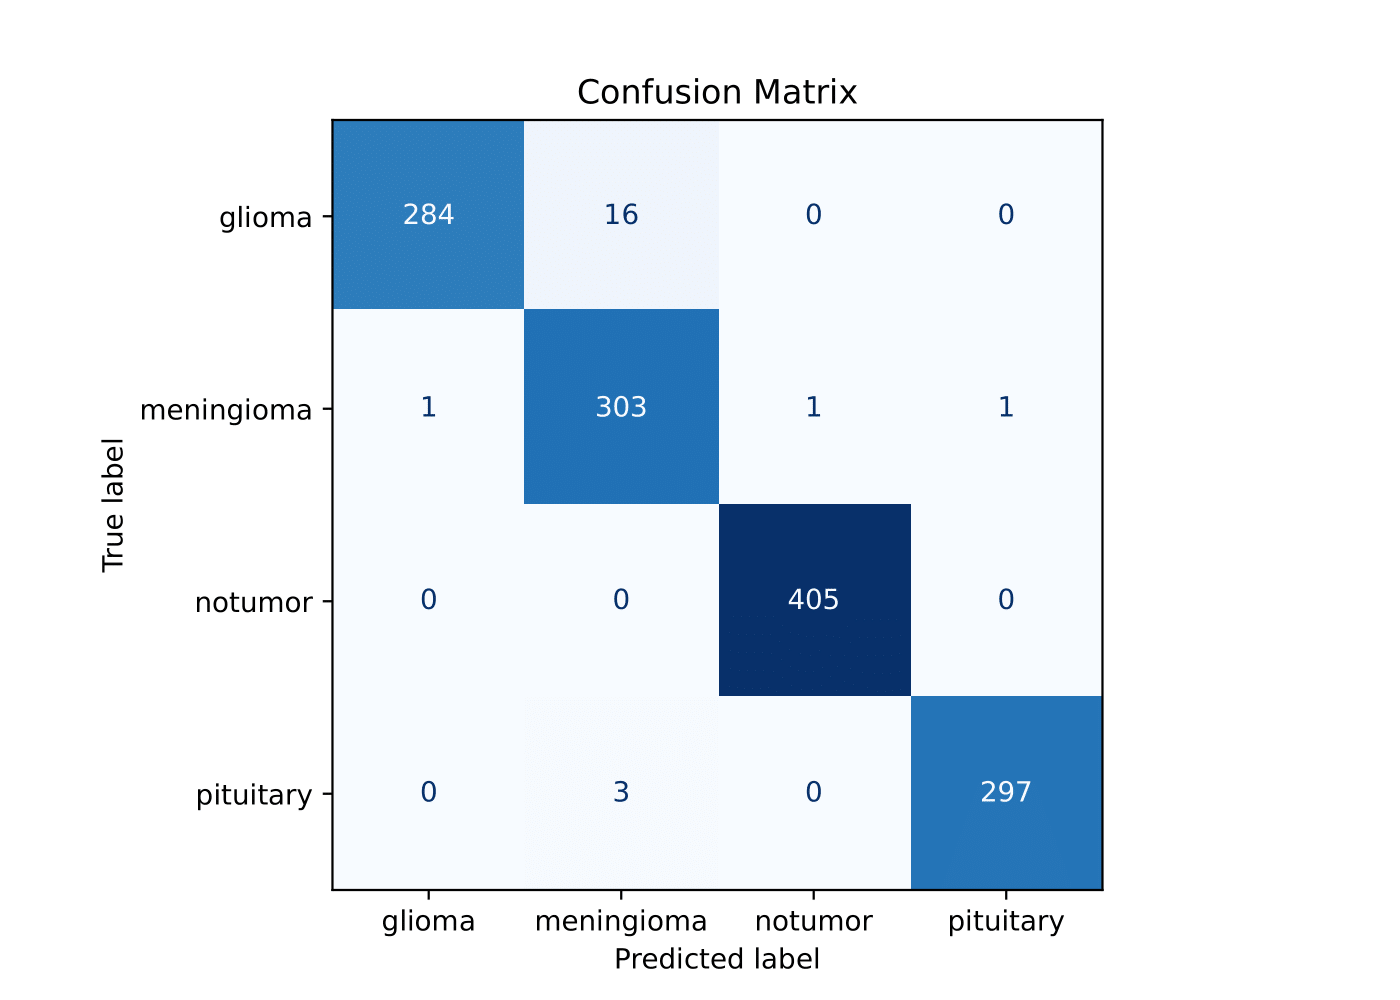
\includegraphics[width=0.6\textwidth]{figures/conf_mat_v3.png}
\caption{Example Confusion Matrix for ViT-B/16}
\label{fig:conf_mat_vit16}
\end{figure}

\item \textbf{ROC Curve}:
A visual representation of model performance across all thresholds. Figure 3 displays a ROC Curve of a ViT-B/16 model trained without data augmentation.
\begin{figure}[H]
\centering
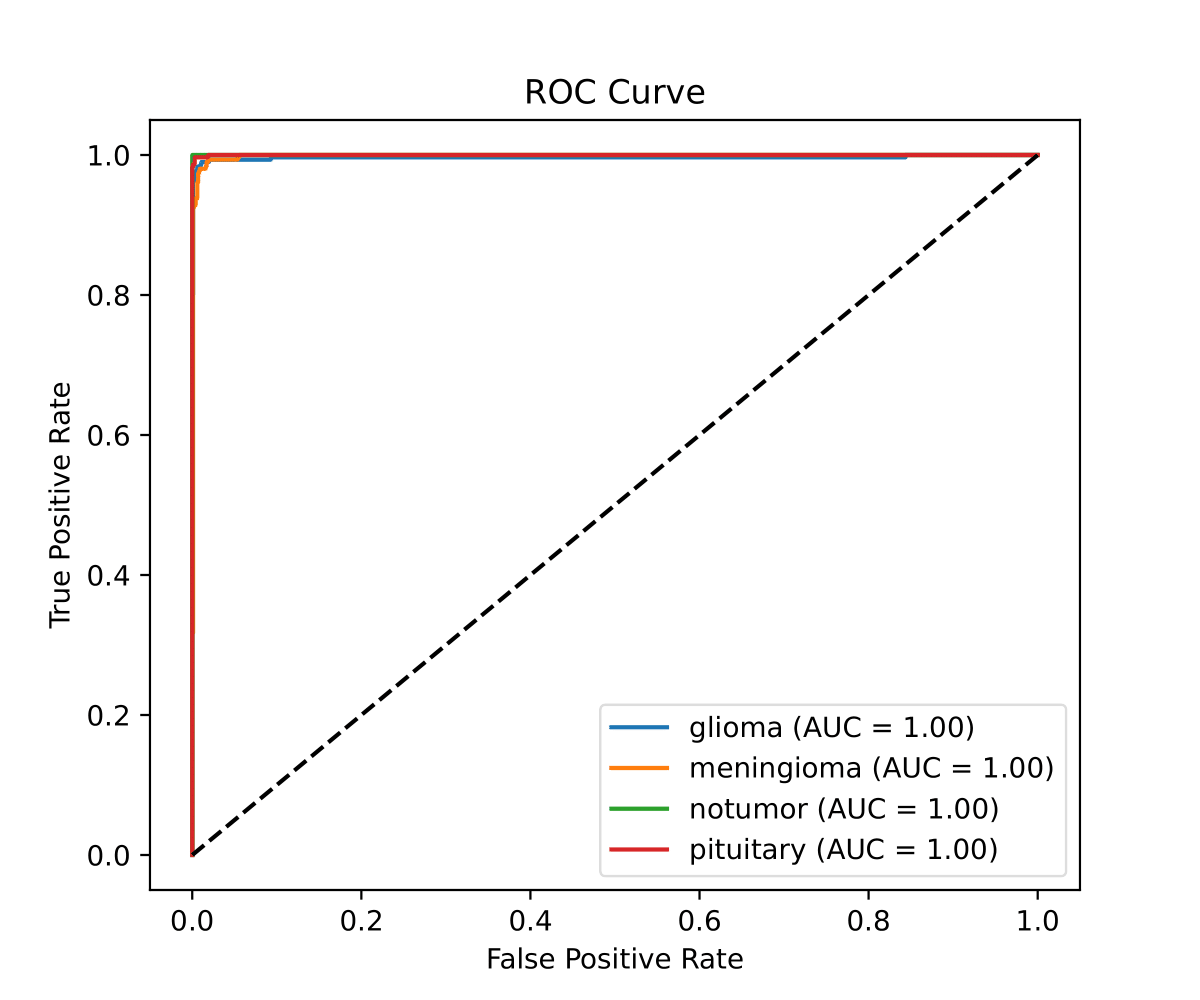
\includegraphics[width=0.6\textwidth]{figures/roc.png}
\caption{Example ROC Curve for ViT-B/16}
\label{fig:roc_vit16}
\end{figure}

\end{itemize}

\section{Software Interface}
\subsection*{Overview}

A custom GUI-based deep learning application was developed to support experimentation, reproducibility, and diagnostic evaluation of brain tumor classification models. Built using Python's built-in Tkinter framework, the software provides an intuitive interface that allows users to configure hyperparameters for model training while viewing results in real-time. This software was developed to improve user accessibility and reproducibility, especially for users without prior programming experience.

\subsection*{Key Features}
\begin{itemize}
\item \textbf{Training Configuration} User-editable fields for model architecture, learning rate, batch size, epochs, and data augmentation.
\item \textbf{Real-Time Console} Dynamic logging of training and testing accuracies with real-time graphical plots.
\item \textbf{Post-Training Diagnostics} After training is completed, a diagnostics panel opens displaying testing results.
\item \textbf{Export Options} Users can export models and export model reports, including metrics, confusion matrices, and ROC curves.
\end{itemize}

\begin{figure}[H]
\centering

\begin{subfigure}[t]{0.32\textwidth}
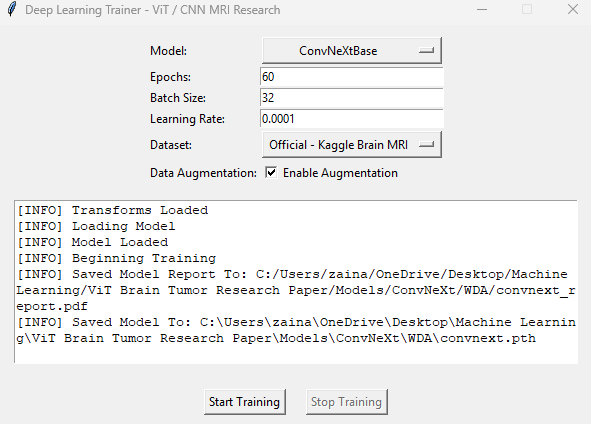
\includegraphics[width=\linewidth]{figures/selection.png}
\caption{Model and Dataset Selection}
\label{fig:gui-window1}
\end{subfigure}
\hfill
\begin{subfigure}[t]{0.32\textwidth}
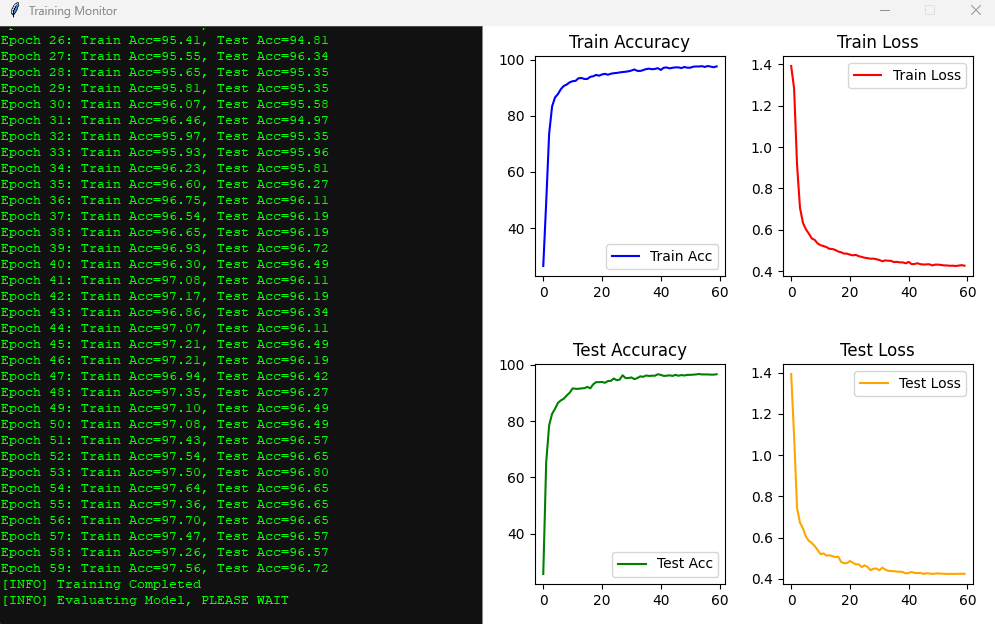
\includegraphics[width=\linewidth]{figures/traininglog.png}
\caption{Real-Time Training Console}
\label{fig:gui-window2}
\end{subfigure}
\hfill
\begin{subfigure}[t]{0.32\textwidth}
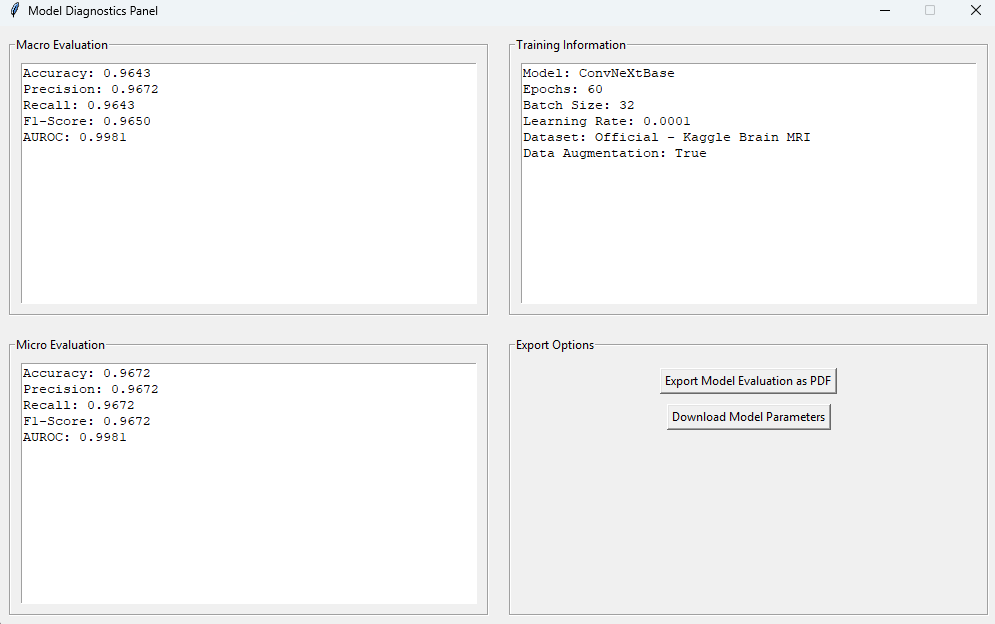
\includegraphics[width=\linewidth]{figures/diagnostics.png}
\caption{Post-Training Diagnostics Panel}
\label{fig:gui-window3}
\end{subfigure}

\caption{Screenshots of the software interface. Users begin by selecting model parameters and dataset (left), monitor training live(center), and view detailed evaluation metrics after training (right).}
\label{fig:gui-windows}
\end{figure}

\begin{figure}[H]
\centering
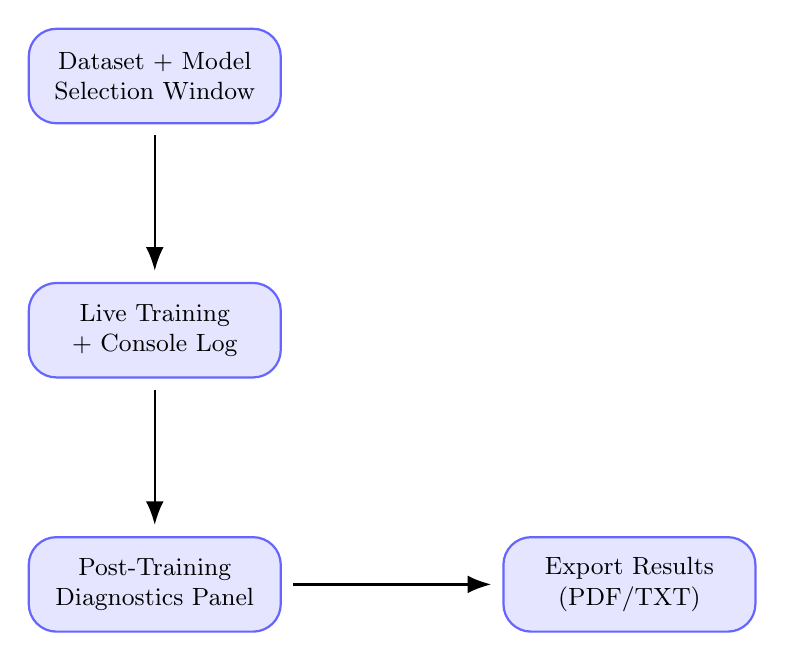
\begin{tikzpicture}[
node distance=2cm and 2.8cm,
every node/.style={font=\small, align=center},
process/.style={rectangle, rounded corners=10pt, draw=blue!60, fill=blue!10, thick, minimum width=3.2cm, minimum height=1.2cm},
arrow/.style={-{Latex[length=3mm]}, thick}
]


\node[process] (load) {Dataset + Model\\ Selection Window};
\node[process, below=of load] (train) {Live Training\\ + Console Log};
\node[process, below=of train] (diagnostics) {Post-Training\\ Diagnostics Panel};
\node[process, right=of diagnostics] (export) {Export Results\\ (PDF/TXT)};


\draw[arrow, shorten >=4pt, shorten <= 4pt] (load) -- (train);
\draw[arrow, shorten >=4pt, shorten <= 4pt] (train) -- (diagnostics);
\draw[arrow, shorten >=4pt, shorten <= 4pt] (diagnostics) -- (export);

\end{tikzpicture}
\caption{Software interface workflow: users progress from dataset/model selection to training, then to diagnostics and export.}
\label{fig:gui-workflow}
\end{figure}

By combining real-time training visualization, easy configuration, and diagnostic output in one interactive and intuitive interface. This effectively bridges the gap between raw machine learning code and practical usability. It serves as an effective research aid and an educational platform for AI-based medical image analysis.


\section{Discussion}

This study revealed that ViT-B/16, EfficientNetB0, and ViT-B/32 achieved the strongest classification performance with test accuracies exceeding 98~\%. Among these models, ViT-B/16 performed best overall, suggesting that small patch sizes and high model capacity enable superior feature extraction in brain MRI classification tasks. Additionally, EfficientNetB0 achieved high performance capabilities despite its relatively lower model complexity compared to other models trained. This highlights the power of efficient CNN architectures when combined with strong inductive biases.

ViT-B/32 demonstrated nearly equivalent performance to ViT-B/16, which indicates that despite larger patch sizes, effective feature extraction can still be conducted. Additionally, this suggests that ViT-B/32 may be a viable alternative for scenarios where computational capacity is limited.

EfficientNetB5, EfficientNetB7, and ConvNextBase produced solid results with accuracies varying between 96 - 97~\%.  However, this highlights that higher model complexity does not translate to improved performance compared to simpler model architectures. Notably, EfficientNetB7 did not yield performance improvements over EfficientNetB0 despite its higher complexity.

SwinV2Base displayed the lowest performance among the evaluated models, with an accuracy of 94~\%. Despite its success in natural vision tasks, its model structure may not have aligned well with the properties of brain MRI data. Additionally, the model's reliance on large-scale pretraining and longer training schedules limited its effectiveness in constrained conditions.

Data augmentation improved performance across nearly all models. While the magnitude of improvement varied by model architecture, the consistent upward trend reinforces the value of augmentation in enhancing generalization and robustness.

ROC Curves for all high-performing models demonstrated strong class separability, with AUROC values consistently above 0.98. The ROC Curves were steep near the origin, confirming low false positive rates (FPR) at high true positive rates (TPR), which is essential in a clinical context where unnecessary alarm must be minimized without compromising sensitivity.

Confusion matrices further revealed that most classification errors occurred between glioma and meningioma classes, as they exhibit overlapping radiological features on MRI scans. Importantly, the number of false negatives was low, but not zero. Despite overall success in preventing false negatives, the presence of false negatives is crucial in medical diagnostics, as failure to detect tumors can delay treatment and impact patient outcomes.

\subsection*{Limitations}

This study was limited to a single, relatively small Brain MRI dataset and did not evaluate cross-instituational generalization or external validation. Additionally, computational resource constraints limited the range of hyperparameter tuning, training duration, and the use of extra data augmentation pipelines. Certain models, such as SwinV2Base, may have underperformed due to insufficient training time or a lack of larger-scale datasets.


\section*{Conclusion}

This study conducted a comparative evaluation of Convolutional Neural Network (CNN) and Vision Transformer (ViT) architectures for multiclass brain tumor classification through brain MRI scans. Among the evaluated models, ViT-B/16, EfficientNetB0, and ViT-B/32 achieved the strongest classification performance with test accuracies exceeding 98~\%. These results suggest that both efficient CNN architectures and transformer-based models can achieve robust diagnostic accuracy in the field of medical imaging diagnostics.

Additionally, the study introduced a custom-built graphical user interface used to streamline model selection, data augmentation, configure model hyperparameters, monitor performance in real-time, and export model reports, including confusion matrices and ROC curves, all without requiring programming expertise. This combination of strong model performance and accessible, easy-to-use software highlights the potential of deep learning to support clinical decision making and education applications in radiology.

\section*{Future Work}
These future research studies can incorporate validation of trained models on more varied datasets, including external institutions and other imaging modalities such as CT and PET. Enhancements can involve ensembling of models, use of tools such as Grad-CAM to localize tumors and visualization, and optimizing hyperparameter search with automated techniques.

\printbibliography

\appendix
\renewcommand{\thesection}{Appendix \Alph{section}}

\clearpage
\pagestyle{fancy}
\fancyhf{} 
\renewcommand{\headrulewidth}{0pt} 
\fancyfoot[C]{Supplementary materials and code available at: \texttt{https://github.com/zaina-ml/brain-mri-classifier}}

\section{Training Recipes}

\begin{table}[H]
\centering
\caption{Training Recipes for All Models}
\begin{tabular}{lcccccc}
\toprule
Model & LR & Batch Size & Epochs & Freeze Epochs & Warmup Epochs \\
\midrule
SwinV2Base       & 1e-4   & 32 & 60 & 5 & 6 \\
ConvNeXtBase     & 1e-4   & 32 & 60 & 5 & 6 \\
ViT-B16          & 1e-4   & 32 & 50 & 5 & 6 \\
ViT-B32          & 1e-4   & 32 & 50 & 5 & 6 \\
EfficientNetB0   & 5e-4   & 32 & 30 & 5 & 3 \\
EfficientNetB5   & 3e-4   & 32 & 50 & 5 & 5  \\
EfficientNetB7   & 1e-4   & 32  & 60 & 5 & 6 \\
\bottomrule
\end{tabular}
\end{table}

\section{Model Architecture Summaries}

\renewcommand{\arraystretch}{1.3}
\begin{table}[H]
\centering
\begin{tabular}{|l|l|c|c|c|l|l|}
\hline
Model & Type & Params (M) & Input Size & Patch/Kernel & Pretrained \\
\hline
EfficientNetB0 & CNN & 5.3  & 224×224 & 3×3        & ImageNet-1k  \\
EfficientNetB5 & CNN & 30.0 & 456×456 & 3×3        & ImageNet-1k  \\
EfficientNetB7 & CNN & 66.0 & 600×600 & 3×3        & ImageNet-1k  \\
ConvNeXt-Base  & CNN & 88.6 & 224×224 & 7×7        & ImageNet-21k  \\
Swin-Base      & Transformer & 87.8 & 224×224 & Shifted 4×4 & ImageNet-21k \\
ViT-B/16       & Transformer & 86.6 & 224×224 & 16×16      & ImageNet-21k  \\
ViT-B/32       & Transformer & 88.6 & 224×224 & 32×32      & ImageNet-21k \\
\hline
\end{tabular}
\caption{Summary of architectures evaluated in this study.}
\end{table}


\section{Training Results for All Models}

\renewcommand{\arraystretch}{1.3}
\begin{table}[H]
\centering
\caption{Macro-averaged performance metrics (\%) for all trained models, with and without data augmentation.}
\label{tab:macro_results}
\begin{tabular}{lcccccc}
\toprule
\textbf{Model} & \textbf{Aug} & \textbf{Accuracy} & \textbf{Precision} & \textbf{Recall} & \textbf{F1 Score} & \textbf{AUROC} \\
\midrule
ViT-B/16       & Yes & 98.25 & 98.37 & 98.25 & 98.28 & 99.91 \\
ViT-B/16       & No  & 98.17 & 98.29 & 98.17 & 98.20 & 99.87 \\
ViT-B/32       & Yes & 97.92 & 98.11 & 97.92 & 97.97 & 99.94 \\
ViT-B/32       & No  & 98.00 & 98.15 & 98.00 & 98.03 & 99.90 \\
EfficientNetB0 & Yes & 98.17 & 98.32 & 98.17 & 98.21 & 99.90 \\
EfficientNetB0 & No  & 98.01 & 98.10 & 98.01 & 98.04 & 99.94 \\
EfficientNetB5 & Yes & 96.95 & 97.22 & 96.95 & 97.03 & 99.76 \\
EfficientNetB5 & No  & 96.69 & 96.83 & 96.69 & 96.74 & 99.78 \\
EfficientNetB7 & Yes & 96.20 & 96.46 & 96.20 & 96.25 & 99.80 \\
EfficientNetB7 & No  & 96.10 & 96.35 & 96.10 & 96.17 & 99.71 \\
ConvNeXtBase   & Yes & 96.43 & 96.72 & 96.43 & 96.50 & 99.81 \\
ConvNeXtBase   & No  & 96.51 & 96.81 & 96.51 & 96.58 & 99.85 \\
SwinV2Base     & Yes & 93.73 & 94.23 & 93.73 & 93.85 & 99.46 \\
SwinV2Base     & No  & 93.66 & 94.20 & 93.66 & 93.77 & 99.45 \\
\bottomrule
\end{tabular}
\end{table}

\section{Appendix: Model Performance Visualizations}

This appendix presents both ROC Curves and Confusion Matrices for each model trained in the study \textbf{with data augmentation} and \textbf{without data augmentation}.


\newcommand{\modelvis}[4]{
\begin{figure}[H]
    \centering
    \begin{subfigure}[t]{0.49\textwidth}
        \centering
        \includegraphics[width=\linewidth]{#1}
        \caption*{Confusion Matrix}
    \end{subfigure}
    \hfill
    \begin{subfigure}[t]{0.49\textwidth}
        \centering
        \includegraphics[width=\linewidth]{#2}
        \caption*{ROC Curve}
    \end{subfigure}
    \caption{#3 -- #4}
\end{figure}
}

\subsection{ConvNeXt-Base}
\subsubsection*{Without Data Augmentation}
\modelvis{figures/model_reports-02.pdf}{figures/model_reports-03.pdf}{ConvNeXt-Base}{No Augmentation}

\subsubsection*{With Data Augmentation}
\modelvis{figures/model_reports-06.pdf}{figures/model_reports-07.pdf}{ConvNeXt-Base}{With Augmentation}

\subsection{EfficientNet-B0}
\subsubsection*{Without Data Augmentation}
\modelvis{figures/model_reports-10.pdf}{figures/model_reports-11.pdf}{EfficientNet-B0}{No Augmentation}

\subsubsection*{With Data Augmentation}
\modelvis{figures/model_reports-14.pdf}{figures/model_reports-15.pdf}{EfficientNet-B0}{With Augmentation}

\subsection{EfficientNet-B5}
\subsubsection*{Without Data Augmentation}
\modelvis{figures/model_reports-18.pdf}{figures/model_reports-19.pdf}{EfficientNet-B5}{No Augmentation}

\subsubsection*{With Data Augmentation}
\modelvis{figures/model_reports-22.pdf}{figures/model_reports-23.pdf}{EfficientNet-B5}{With Augmentation}

\subsection{EfficientNet-B7}
\subsubsection*{Without Data Augmentation}
\modelvis{figures/model_reports-26.pdf}{figures/model_reports-27.pdf}{EfficientNet-B7}{No Augmentation}

\subsubsection*{With Data Augmentation}
\modelvis{figures/model_reports-30.pdf}{figures/model_reports-31.pdf}{EfficientNet-B7}{With Augmentation}

\subsection{SwinV2-Base}
\subsubsection*{Without Data Augmentation}
\modelvis{figures/model_reports-34.pdf}{figures/model_reports-35.pdf}{SwinV2-Base}{No Augmentation}

\subsubsection*{With Data Augmentation}
\modelvis{figures/model_reports-38.pdf}{figures/model_reports-39.pdf}{SwinV2-Base}{With Augmentation}

\subsection{ViT-B/16}
\subsubsection*{Without Data Augmentation}
\modelvis{figures/model_reports-42.pdf}{figures/model_reports-43.pdf}{ViT-B/16}{No Augmentation}

\subsubsection*{With Data Augmentation}
\modelvis{figures/model_reports-46.pdf}{figures/model_reports-47.pdf}{ViT-B/16}{With Augmentation}

\subsection{ViT-B/32}
\subsubsection*{Without Data Augmentation}
\modelvis{figures/model_reports-50.pdf}{figures/model_reports-51.pdf}{ViT-B/32}{No Augmentation}

\subsubsection*{With Data Augmentation}
\modelvis{figures/model_reports-54.pdf}{figures/model_reports-55.pdf}{ViT-B/32}{With Augmentation}

\clearpage
\pagestyle{plain}

\end{document}
